\documentclass[12pt,a4paper]{book}

% ----- Encodage & langues -----
\usepackage[utf8]{inputenc}    % Encodage UTF-8
\usepackage[T1]{fontenc}       % Meilleure gestion des accents
\usepackage[french]{babel}     % Langue du document (français)

% ----- Police -----
\usepackage{lmodern}           % Police Latin Modern (propre et lisible)
%\usepackage{mathpazo}         % Option : police Palatino
%\usepackage{times}            % Option : police Times

% ----- Mise en page -----
\usepackage[a4paper,margin=2.5cm]{geometry} % Marges

% ----- Liens cliquables -----
\usepackage[hidelinks]{hyperref} % Liens URL et références
\hypersetup{
    colorlinks=true,
    linkcolor=blue,
    urlcolor=cyan,
    citecolor=red
}

% ----- Table des matières -----
\setcounter{tocdepth}{2} % Profondeur de la ToC (sections, sous-sections, etc.)

% ----- Autres utiles -----
\usepackage{graphicx}     % Pour insérer des images
\usepackage{amsmath,amssymb} % Maths
\usepackage{enumitem}     % Listes personnalisées
\usepackage{fancyhdr}     % En-têtes et pieds de page
\usepackage{setspace}     % Interligne
\onehalfspacing           % Interligne 1.5
\usepackage{titling}
\usepackage{epigraph}
\usepackage[most]{tcolorbox}
\usepackage{xcolor}
\usepackage{mdframed}
\usepackage{textcomp}

% Définition d'une citation décorative
\newmdenv[
    backgroundcolor=gray!8,    % Fond gris très clair
    linewidth=0pt,             % Pas de bordure
    leftmargin=0pt,            % Supprime les marges automatiques
    rightmargin=0pt,
    innerleftmargin=2em,       % Marge interne gauche
    innerrightmargin=2em,      % Marge interne droite
    innertopmargin=1em,
    innerbottommargin=1em,
    roundcorner=5pt,
    font=\itshape\centering,   % Italique et centré
    align=center,              % Centre la boîte elle-même
    userdefinedwidth=0.7\textwidth  % Largeur définie (70% du texte)
]{citationmd}


% ----- Début du document -----

\begin{document}

\begin{titlepage}
    \centering
    \vspace{1cm}
    \Huge
    \textbf{L'Odyssée de l'Intelligence Artificielle}
    
    \begin{figure}[h]
        \centering
        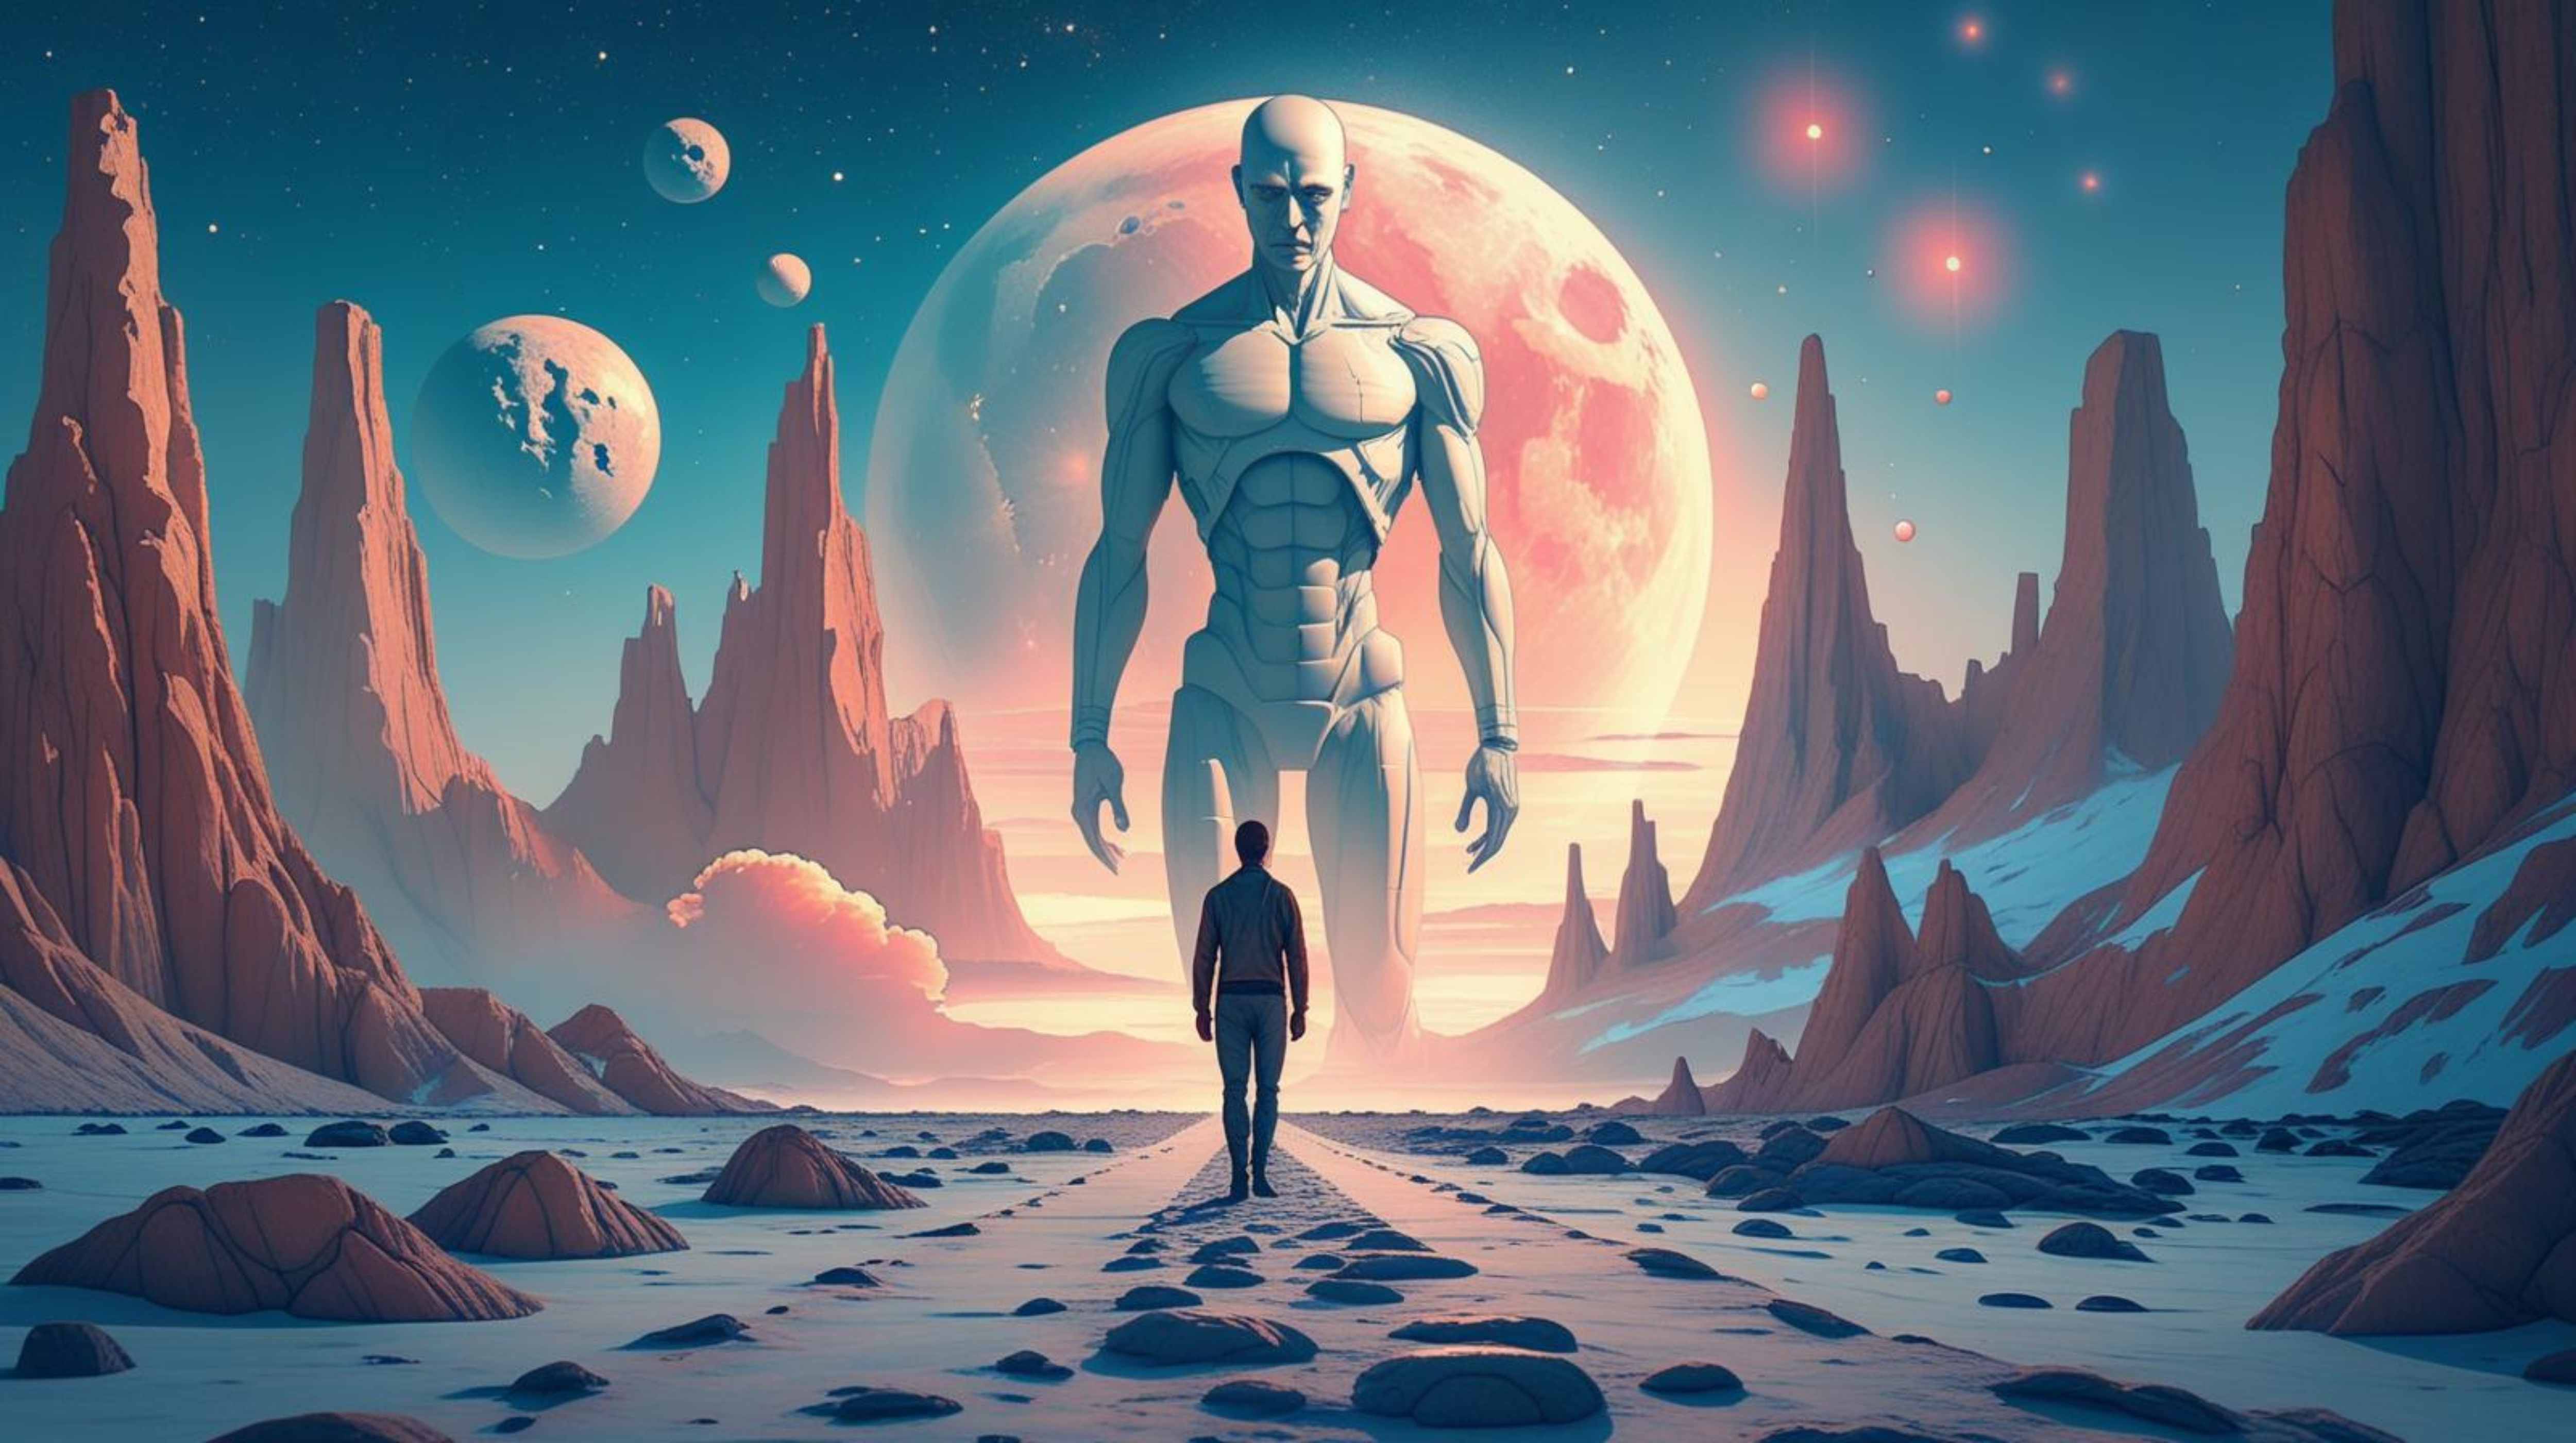
\includegraphics[width=1\textwidth]{images/partie1/odysse.png}
    \end{figure}

    \vspace{0.5cm}
    
    \LARGE
    \textit{Des Origines Anthropologiques aux Horizons Contemporains}
    
    \vspace{2cm}

    \Large
    Romuald Courtois
    
    \vspace{2cm}
            
    \large
    2025

\end{titlepage}

\newpage
\pagestyle{empty}

\begin{center}
2025 Romuald Courtois

\bigskip

Tous droits réservés. Aucune partie de ce livre ne peut être reproduite, stockée dans un système de récupération, ou transmise sous aucune forme ni aucun moyen, électronique, mécanique, photocopie, enregistrement ou autre, sans l'autorisation écrite préalable de l'auteur, sauf dans les cas prévus par la loi (citations, critiques, usages pédagogiques).

\bigskip

ISBN : [Votre numéro ISBN]

\bigskip

Dépôt légal : 23/09/2025

\bigskip

Édition : Auto-édition

\bigskip

Adresse de l'auteur / de l'éditeur :\\
151 Traverse de la Gouffonne, 13009 MARSEILLE

\bigskip

Pour obtenir une autorisation de reproduction ou pour toute question relative aux droits, veuillez contacter :\\
romuald.courtois.at.proton.me

\bigskip

Les noms de marques, logos, produits ou institutions mentionnés dans ce livre sont la propriété de leurs détenteurs respectifs.

\bigskip

La couverture a été réalisée par : Romuald Courtois
\end{center}

\newpage
\pagestyle{empty}
\chapter*{Préface} % Titre sans numéro
\addcontentsline{toc}{chapter}{Préface}  % Ajoute la préface à la table des matières
Dans chaque avancée technologique, dans chaque progrès de la pensée humaine, se cache un paradoxe fascinant : celui de l'éternel fainéant ambitieux. Ce livre s'articule autour de cette idée directrice, selon laquelle l'humanité, portée par une ambition immense, cherche depuis toujours à alléger ses efforts par l'externalisation de ses capacités — qu'elles soient physiques, intellectuelles ou créatives. Nous sommes à la fois poussés par la paresse, ce désir de faciliter notre quotidien, et par une soif infinie d'innovation, de conquête intellectuelle.
\\ \\
L'histoire de l'intelligence artificielle est de fait une illustration parfaite de ce double mouvement. Depuis les premiers automates antiques jusqu'aux réseaux neuronaux profonds d'aujourd'hui, cette quête révèle non seulement notre envie d'économiser l'énergie humaine, mais aussi notre rêve de transcender nos limites cognitifs. Ce livre retrace cette odyssée passionnante, mêlant récits historiques, analyses techniques et réflexions éthiques.
\\ \\
À travers la figure de ce "fainéant ambitieux", j'espère porter un regard à la fois critique et bienveillant sur les innovations majeures, en montrant comment chaque invention est à la fois un outil pour réduire l'effort et un levier d'ambition démesurée. Il invite le lecteur à comprendre que derrière chaque progrès, derrière chaque machine intelligente, il y a une humanité impatiente qui cherche inlassablement à se simplifier la vie… tout en repoussant ses propres frontières.
\\ \\
Que cet ouvrage nourrisse la curiosité, stimule la réflexion et éclaire le chemin vers une intelligence artificielle enfin alignée avec nos valeurs et nos besoins profonds.
\\ \\
\begin{citationmd}
\centering\itshape\large
"L'homme est un éternel fainéant ambitieux : trop paresseux pour accepter la répétition, trop intelligent pour accepter l'inefficacité. C'est cette contradiction qui nous a menés de l'outil de pierre aux neurones artificiels."
\end{citationmd}
 
\pagestyle{empty}
\tableofcontents

\newpage
\pagestyle{plain}
\chapter*{Introduction}
\addcontentsline{toc}{chapter}{Introduction}

L'intelligence artificielle, souvent perçue comme une révolution contemporaine, est en réalité l'aboutissement d'une quête profondément ancrée dans l'histoire même de l'humanité, bien avant l'invention des premiers outils sophistiqués. Pour comprendre pleinement cette trajectoire, il faut remonter jusqu'aux origines de notre espèce, à ce moment clé où nos ancêtres ont commencé à se redresser, posant ainsi les premières pierres d'un cheminement qui allait transformer non seulement leur corps, mais aussi leur esprit.
\\ \\
Le passage à la bipédie, il y a plus de 4 millions d'années, a libéré les mains tout en stimulant les possibilités cognitives, ouvrant la voie à la fabrication d'outils rudimentaires. Ces premières externalisations des fonctions physiques incarnent déjà la dynamique que l'on retrouve dans l'intelligence artificielle : réduire la charge corporelle ou mentale par l'usage d'artefacts externes. Cette ambition de « paresse créative » est à l'origine de toutes les technologies, et en filigrane de l'émergence des processus cognitifs complexes qui caractérisent notre espèce.
\\ \\
Ce livre propose donc de retracer l'odyssée de l'IA en partant de ce moment fondamental où l'humanité s'est levée, au propre et au figuré, jusqu'aux dernières innovations numériques actuelles. Il s'agit d'un voyage mêlant anthropologie, technologie, philosophie et éthique, qui éclaire comment, à chaque époque, le désir d'alléger l'effort s'est conjugué à une ambitieuse vision d'extension des capacités humaines. 
\\ \\
À travers la notion de \textit{"l'éternel fainéant ambitieux"}, vous découvrirez comment cette dualité originelle continue de guider nos inventions et leurs implications. Ce n'est pas seulement une histoire de machines, mais celle du regard humain sur lui-même, sur ses potentialités et ses limites. 
\\ \\
Bienvenue dans cette plongée aux origines, à la source de toute intelligence, humaine et artificielle.

\newpage

\part{GENÈSE ET FONDEMENTS HISTORIQUES}

\chapter{Genèse Anthropologique - L'Éveil du Fainéant}
\section{Principe d'économie d'énergie cognitive}
\section{Bipédie et libération cognitive (4 Ma - 200 000 ans)}
\section{Premiers outils lithiques et externalisation motrice}
\section{Révolution cognitive et pensée symbolique (70 000 - 10 000 ans)}
\section{Néolithique, spécialisation et division du travail}
\section{L'ambition par la paresse : Extensions des possibles}

\chapter{Civilisations Antiques et Mécanisation Primitive}
\section{Mésopotamie - Calculs, abaques et premiers algorithmes}
\section{Égypte - Mathématiques, ingénierie et automatisation}
\section{Grèce - Logique, philosophie et automates mécaniques}
\section{Rome - Ingénierie, hydraulique et machines complexes}
\section{Héron d'Alexandrie - Premier ingénieur de l'automation}
\section{Machine d'Anticythère - Ordinateur analogique antique}

\chapter{Synthèses Orientales et Renaissance Islamique}
\section{Inde - Mathématiques, logique et premiers concepts algorithmiques}
\section{Chine ancienne - Boulier, poudre et automates mécaniques}
\section{Systèmes d'irrigation chinois - Automatisation hydraulique}
\section{Islam - Traductions, mathématiques et premiers ordinateurs mécaniques}
\section{Al-Jazari - Livre de la connaissance des procédés mécaniques}
\section{Avicenne et Averroès - Logique médiévale et formalisation}
\section{Transmission vers l'Europe - Textes, écoles et premiers penseurs}

\chapter{Renaissance Européenne et Révolution Scientifique}
\section{Léonard de Vinci - Automates et machines programmables}
\section{Horlogerie suisse - Miniaturisation et précision mécanique}
\section{Révolution astronomique - Kepler, calculs et précision}
\section{Pascal et Leibniz - Premières machines à calculer}
\section{Leibniz et le calcul binaire - Fondements de l'informatique}
\section{Newton et la mathématisation du monde}

\chapter{Siècle des Lumières et Mécanisation}
\section{Descartes et l'animal-machine - Philosophie mécaniste}
\section{La Mettrie - L'Homme-Machine et matérialisme}
\section{Automates de Vaucanson et illusion de vie}
\section{Automates Jaquet-Droz - Écrivain, Dessinateur, Musicien}
\section{Encyclopédie et diffusion des techniques}
\section{Révolution industrielle - Métiers mécaniques et automation}
\section{Jacquard - Programmation par cartes perforées}

\chapter{XIXe Siècle - Émergence de l'Information}
\section{Babbage et Lovelace - Machines analytiques}
\section{Ada Lovelace - Premier algorithme et vision créative de l'IA}
\section{Boole - Algèbre logique et fondements booléens}
\section{De Morgan et logique des relations}
\section{Maxwell, thermodynamique et théorie de l'information}
\section{Télégraphie, codes et transmission}
\section{Herman Hollerith - Machines à cartes perforées et recensement}

\part{NAISSANCE ET DÉVELOPPEMENT DE L'IA MODERNE}

\chapter{XXe Siècle - Fondements Théoriques}
\section{Russell et Whitehead - Principia Mathematica}
\section{Hilbert et formalisme mathématique}
\section{Gödel - Limites de la démonstration automatique}
\section{Church et lambda-calcul}
\section{Turing - Calculabilité et machines universelles}
\section{Test de Turing - Critère d'intelligence artificielle}
\section{Von Neumann - Architecture et automates cellulaires}

\chapter{Naissance Officielle de l'IA (1940-1960)}
\section{McCulloch-Pitts et neurones formels}
\section{Wiener et cybernétique}
\section{Shannon et théorie de l'information}
\section{Premiers ordinateurs - ENIAC, UNIVAC, IBM 701}
\section{Conférence de Dartmouth et manifeste fondateur}
\section{John McCarthy - Invention du terme "Intelligence Artificielle"}
\section{Marvin Minsky - Vision de l'IA symbolique}

\chapter{Première Génération - Optimisme Symbolique (1956-1974)}
\section{Logic Theorist et résolution automatique}
\section{General Problem Solver - Newell et Simon}
\section{Perceptron et apprentissage connexionniste}
\section{ELIZA - Premier chatbot thérapeutique}
\section{LISP et programmation symbolique}
\section{PROLOG - Programmation logique}
\section{Premiers systèmes experts et bases de connaissances}
\section{Shakey le robot - Intégration perception-action}
\section{Vision par ordinateur - Premiers succès et limites}

\chapter{Premier Hiver et Remises en Question (1974-1980)}
\section{Rapport Lighthill et crise de confiance}
\section{Limites des perceptrons (Minsky-Papert)}
\section{Complexité computationnelle et problèmes NP}
\section{Explosion combinatoire - Limites pratiques des systèmes}
\section{Échec des promesses et réduction des financements}
\section{Repositionnement académique et industriel}

\chapter{Renaissance des Systèmes Experts (1980-1990)}
\section{MYCIN et diagnostic médical automatisé}
\section{DENDRAL et analyse chimique}
\section{XCON/R1 - Premier succès commercial (DEC)}
\section{Ingénierie de la connaissance et ontologies}
\section{Langages spécialisés - OPS5, KEE, ART}
\section{Machines Lisp - Symbolics, LMI}
\section{Marché commercial et désillusions}
\section{Effondrement 1987 - "Mardi noir de l'IA"}

\chapter{Révolution Statistique et Second Hiver (1987-1997)}
\section{Causes du second effondrement}
\section{Réseaux de neurones et rétropropagation}
\section{Support Vector Machines - Vapnik}
\section{Réseaux bayésiens et raisonnement probabiliste}
\section{Algorithmes génétiques - John Holland}
\section{Machine Learning et approches data-driven}
\section{Hidden Markov Models - Applications vocales}
\section{Deep Blue vs Kasparov - Calcul brut vs intuition (1997)}

\part{RÉVOLUTION CONTEMPORAINE ET IMPACTS SOCIÉTAUX}

\chapter{Internet et Renaissance des Données (1997-2010)}
\section{Explosion du Web - Données massives}
\section{Web sémantique et ontologies distribuées}
\section{Big Data et nouveaux paradigmes d'apprentissage}
\section{Google et PageRank - IA comme service}
\section{Gmail spam filter - Apprentissage bayésien à grande échelle}
\section{Réseaux sociaux et intelligence collective}
\section{Geoffrey Hinton - Réveil du deep learning (2006)}
\section{GPU et calcul parallèle - CUDA NVIDIA}
\section{ImageNet - Benchmark vision par ordinateur}

\chapter{Deep Learning et Révolution Connexionniste (2010-2016)}
\section{Percée 2012 - Confluence de facteurs}
\section{AlexNet et renaissance des CNN (2012)}
\section{VGGNet - Architecture profonde (2014)}
\section{ResNet - Connexions résiduelles (2015)}
\section{GANs et génération de contenu artificiel}
\section{RNN, LSTM et modélisation séquentielle}
\section{Attention mechanisms - Bahdanau (2014)}
\section{Deep Q-Networks - Apprentissage par renforcement}
\section{TensorFlow et PyTorch - Démocratisation des outils}
\section{Révolution Transformers et mécanismes d'attention}

\chapter{IA Générative et Démocratisation (2017-2025)}
\section{"Attention Is All You Need" - Architecture Transformer (2017)}
\section{BERT - Compréhension bidirectionnelle (2018)}
\section{GPT et génération de texte à grande échelle}
\section{GPT-2 - Controverse "trop dangereux" (2019)}
\section{GPT-3 - Scaling laws et capacités émergentes (2020)}
\section{DALL-E et création d'images automatisée}
\section{Midjourney et Stable Diffusion - Démocratisation}
\section{ChatGPT et interface conversationnelle grand public (2022)}
\section{GPT-4 - Capacités multimodales (2023)}
\section{Codex et programmation assistée par IA}
\section{Agents autonomes - AutoGPT et planification}

\chapter{Succès Médiatisés et Révolutions Sectorielles}
\section{Netflix Recommandations - Révolution de la personnalisation (2006)}
\section{Spotify Discover Weekly - Algorithmes musicaux (2015)}
\section{AlphaGo vs Lee Sedol - Maîtrise du jeu de Go (2016)}
\section{AlphaZero - Apprentissage sans données humaines (2017)}
\section{AlphaFold - Révolution en biologie structurale (2020)}
\section{AlphaFold 3 - Prix Nobel de chimie induit par IA (2024)}
\section{GitHub Copilot - IA collaborative en programmation (2021)}
\section{Waymo - Milliards de km autonomes sans accident}
\section{GPT-4 médical - Performances niveau expert}

\chapter{Échecs Médiatisés et Leçons Critiques}
\section{Accident Tesla Autopilot - Limites de la conduite autonome (2016)}
\section{Uber Tempe - Accident mortel piéton (2018)}
\section{Tay de Microsoft - Dérapage raciste en 24h (2016)}
\section{Reconnaissance faciale biaisée - Amazon Rekognition (2018)}
\section{IBM Watson Health - Échec médical et fermeture (2022)}
\section{Google Flu Trends - Prédictions erronées (2013)}
\section{Zillow iBuying - Algorithmes immobiliers défaillants (2021)}
\section{ChatGPT et hallucinations juridiques (2023)}
\section{McDonald's Drive-AI - Abandon commercial (2024)}
\section{Boeing 737 MAX - MCAS et accidents (2018-2019)}
\section{Knight Capital - Bug algorithmique à 440M$ (2012)}

\chapter{IA Militaire et Géopolitique}
\section{Systèmes d'armes autonomes (LAWS) et débat éthique}
\section{Drones Kargu-2 - Premier kill autonome confirmé (Libye 2020)}
\section{Projet Maven - Contestation Google (2018)}
\section{Cyberguerre et IA défensive/offensive}
\section{Stuxnet - Précurseur cyber-arme (2010)}
\section{Course géopolitique USA-Chine-Europe}
\section{Initiative américaine - NSCAI et leadership IA}
\section{Plan chinois - AI 2030 et domination}
\section{Souveraineté européenne - GAIA-X, Mistral AI}
\section{Surveillance de masse et contrôle social}
\section{Système de crédit social chinois}
\section{Reconnaissance faciale Clearview AI}

\part{DIMENSIONS HUMAINES ET PROSPECTIVE}

\chapter{IA et Santé - Révolution Médicale}
\section{Diagnostic par imagerie - Radiologie, dermatologie, ophtalmologie}
\section{Drug discovery - Molécules thérapeutiques par IA}
\section{Chirurgie robotique - Da Vinci, précision augmentée}
\section{Télémédecine et assistants diagnostiques}
\section{Épidémiologie - Modélisation COVID-19}
\section{Thérapies personnalisées - Médecine de précision}
\section{Limites et échecs - IBM Watson Oncology}

\chapter{Approches Bio-Inspirées et Active Inference}
\section{Friston et Free Energy Principle}
\section{Active Inference et anticipation prédictive}
\section{Neurosciences computationnelles et modélisation cérébrale}
\section{Réseaux de neurones évolutionnistes}
\section{Neuromorphic Computing - Puces TrueNorth, Loihi}
\section{Spiking Neural Networks - Bio-réalisme événementiel}
\section{Reservoir Computing - Économie computationnelle}

\chapter{Facteurs Humains et Ergonomie Cognitive}
\section{IHM et interfaces adaptatifs}
\section{Lecture des intentions par eye-tracking}
\section{Brain-Computer Interfaces non-invasives}
\section{Cognition énactive et robotique incarnée}
\section{Charge cognitive et optimisation des performances}
\section{Explainability (XAI) - IA interprétable}
\section{Trust calibration - Confiance appropriée}
\section{Human-in-the-loop - Supervision humaine optimale}

\chapter{Interfaces Cerveau-IA et Augmentation Cognitive}
\section{Neuralink et interfaces implantées - Progrès et risques}
\section{Synchron - Implants vasculaires moins invasifs}
\section{Kernel - Interfaces optiques non-invasives}
\section{Délestage cognitif - Dépendance et atrophie des capacités}
\section{Memory augmentation - Prothèses mnésiques}
\section{IA thérapeutique - Santé mentale, autisme, réhabilitation}
\section{Stimulation cérébrale profonde assistée par IA}
\section{Biais cognitifs humains reproduits par l'IA}
\section{Effets psychologiques - Anthropomorphisation, attachement}

\chapter{Les Oubliés de la Révolution IA}
\section{Pionniers invisibles - Femmes en IA (Ada Lovelace revisitée)}
\section{Grace Hopper - COBOL et compilation}
\section{Fei-Fei Li - ImageNet et démocratisation}
\section{Contributeurs non-occidentaux souvent occultés}
\section{Yoshua Bengio, Yann LeCun - Pionniers du deep learning}
\section{Populations rurales et seniors face à l'IA}
\section{Illectronisme - Nouvelle forme d'illettrisme}
\section{Travailleurs du clic et main-d'œuvre cachée}
\section{Annotateurs kenyans de ChatGPT - Conditions dégradées}
\section{Modérateurs de contenu - Trauma psychologique}
\section{Fracture Nord-Sud - Accès inégal aux modèles}

\chapter{Transformation Sociétale et Économique}
\section{Remplacement d'emplois et nouvelles professions}
\section{Automatisation différentielle - Cols blancs vs bleus}
\section{Métiers émergents - Prompt engineer, AI ethics officer}
\section{Fracture numérique et inégalités d'accès}
\section{IA générative et propriété intellectuelle}
\section{Procès copyright - NYT vs OpenAI, Getty vs Stability}
\section{Revenu universel - Nécessité face à l'automation}
\section{Économie de l'attention et manipulation comportementale}
\section{Dopamine design - Exploitation des biais cérébraux}
\section{Économie de la data - Nouveau pétrole}

\chapter{IA Créative et Patrimoine Culturel}
\section{IA générative artistique - DALL-E, Midjourney, Stable Diffusion}
\section{Musique générée par IA - Suno, Udio}
\section{Littérature et IA - GPT-poetry, co-écriture}
\section{Victoires littéraires d'IA - Prix et controverses}
\section{Préservation du patrimoine - Numérisation, restauration virtuelle}
\section{Notre-Dame - Scan 3D et reconstruction}
\section{Scrolls d'Herculanum - Déchiffrage par IA}
\section{Déformation historique - Risques pour la mémoire collective}
\section{Falsification historique - Deepfakes de figures historiques}

\chapter{Convergences Technologiques Émergentes}
\section{Informatique quantique et IA}
\section{D-Wave, IBM Q, Google Sycamore - État de l'art}
\section{Algorithmes quantiques pour ML}
\section{IA + Biotechnologies - Drug discovery, thérapies géniques}
\section{CRISPR assisté par IA - Édition génomique précise}
\section{IA + Nanotechnologies - Smart materials, médecine régénérative}
\section{Internet des Objets intelligent - Edge computing, IA embarquée}
\section{5G/6G et IA distribuée}
\section{Digital twins - Jumeaux numériques prédictifs}

\chapter{IA et Environnement}
\section{Empreinte carbone de l'IA - Datacenters, consommation énergétique}
\section{Entraînement GPT-3 - 1287 MWh, 552 tonnes CO₂}
\section{Refroidissement datacenters - Innovations liquides}
\section{IA pour le climat - Modélisation, smart grids, optimisation}
\section{Prédiction climatique - Modèles haute résolution}
\section{Agriculture de précision - Drones, capteurs, optimisation}
\section{Economie circulaire et IA prédictive}
\section{Maintenance prédictive - Réduction du gaspillage}
\section{Obsolescence et e-waste des systèmes IA}
\section{Recyclage des GPUs - Enjeux des terres rares}

\chapter{Paradigmes Alternatifs et Techniques Redécouvertes}
\section{Techniques pré-deep learning redécouvertes}
\section{Capsule Networks - Hinton (2017)}
\section{Neural Turing Machines - Mémoire externe}
\section{IA symbolique hybride - Retour du raisonnement logique}
\section{Neuro-symbolique - Meilleur des deux mondes}
\section{Bio-computing - ADN, protéines comme processeurs}
\section{Calcul moléculaire - Portes logiques biologiques}
\section{IA frugale - Algorithmes low-tech, edge computing}
\section{TinyML - IA sur microcontrôleurs}
\section{Pruning et quantization - Compression de modèles}

\chapter{Langages et Infrastructure de l'IA}
\section{Évolution des langages - LISP, PROLOG, Python}
\section{Frameworks modernes - TensorFlow, PyTorch, JAX}
\section{Hardware spécialisé - GPU, TPU, NPU}
\section{Architectures cloud - AWS SageMaker, Azure ML, Google Vertex}
\section{MLOps - Industrialisation du ML}
\section{Open source vs propriétaire - Tensions}

\chapter{Dérives, Abus et Risques Systémiques}
\section{Deepfakes et manipulation de l'information}
\section{Cas politique - Deepfakes électoraux}
\section{Pornographie deepfake - Victimisation}
\section{Propagation automatisée de la désinformation}
\section{Bots coordonnés - Amplification algorithmique}
\section{Surveillance de masse et atteintes à la vie privée}
\section{Reconnaissance faciale en temps réel}
\section{Scrapage massif - Clearview AI, PimEyes}
\section{Automatisation des cyberattaques et armes numériques}
\section{Phishing assisté par GPT}
\section{Malware auto-adaptatif}
\section{Discrimination algorithmique et exacerbation des inégalités}
\section{Biais raciaux - Justice prédictive (COMPAS)}
\section{Sexisme algorithmique - Recrutement, crédit}
\section{Effets sur la santé mentale et dépendance aux systèmes IA}
\section{Addiction aux recommandations}
\section{Isolement social - Relations parasociales avec IA}

\chapter{Confidentialité et Sécurité des Données dans l’IA}

\section{Cadre Réglementaire et Légal}
\subsection{Règlement général sur la protection des données (RGPD)}
\subsection{AI Act et régulation spécifique à l’intelligence artificielle}
\subsection{Le droit à l’oubli et les obligations des acteurs IA}

\section{Défis Techniques en Protection des Données}
\subsection{Anonymisation, pseudonymisation et leurs limites}
\subsection{Cryptographie avancée appliquée à l’IA : chiffrement homomorphe, calcul multipartite sécurisé}
\subsection{Attaques adversariales et vulnérabilités des modèles IA}

\section{Risques et Menaces sur la Confidentialité}
\subsection{Fuites de données et piratage de modèles}
\subsection{Extraction illégale de données personnelles via modèles d’IA}
\subsection{Utilisation non consentie des données dans l’entraînement des modèles}

\section{Solutions et Meilleures Pratiques}
\subsection{Privacy by design et confidentialité différentielle}
\subsection{Audits de sécurité et lutte contre les biais algorithmiques}
\subsection{Gouvernance des données et rôle des délégués à la protection des données (DPO)}

\section{Cas d’Études et Incidents Marquants}
\subsection{Scandales de violation de vie privée liés à l’IA}
\subsection{Cyberattaques sur infrastructures critiques IA}


\chapter{Débats Philosophiques et Conscience Artificielle}
\section{Conscience et qualia - Le problème difficile}
\section{Test de Turing moderne - Suffisance ou obsolescence ?}
\section{Chambre chinoise de Searle - Critique philosophique}
\section{Panpsychisme computationnel}
\section{Sentience des LLMs - Affaire Blake Lemoine (Google)}
\section{Droits des IA - Statut juridique futur}
\section{Éthique de la création - Responsabilité des concepteurs}

\chapter{Évolution de l'Éthique et Gouvernance}
\section{Principes fondateurs et chartes d'intention}
\section{Principes d'Asilomar (2017)}
\section{Montreal Declaration (2018)}
\section{RGPD, AI Act et régulation européenne}
\section{AI Act - Première loi globale (2024)}
\section{Approche par niveaux de risque}
\section{Gouvernance mondiale et coopération internationale}
\section{ONU et IA - Propositions de gouvernance}
\section{OCDE - Principes sur l'IA}
\section{Justice algorithmique et lutte contre les biais}
\section{Audits algorithmiques obligatoires}
\section{Fairness metrics - Définitions et limites}
\section{Transparence des modèles - Open weights vs closed}

\chapter{Vers l'AGI et Singularité Technologique}
\section{Définitions et critères de l'AGI}
\section{Chronologie probable - Prédictions d'experts}
\section{Singularité technologique - Kurzweil et critiques}
\section{Intelligence explosive - Scénarios de décollage}
\section{Alignement de valeurs - Problème de contrôle}
\section{Mesa-optimization - Optimiseurs internes}
\section{Orthogonalité - Intelligence ≠ Bienveillance}
\section{Paperclip maximizer - Optimisation perverse}

\chapter{Course Concurrentielle et Moloch}
\section{Moloch de l'IA - Dynamique compétitive}
\section{Course aux armements IA - Équilibre de Nash négatif}
\section{Dilemme du prisonnier itéré}
\section{Coordination internationale - Nécessité et difficultés}
\section{Ralentissement concerté - Propositions et critiques}
\section{Lettre ouverte 2023 - Pause développement IA}
\section{Accélérationnisme vs décélérationnisme}

\chapter{Post-Humanisme et Transhumanisme}
\section{Amélioration cognitive - Limites éthiques}
\section{Uploading de conscience - Faisabilité technique}
\section{Cyborgs et hybridation - Continuité humain-machine}
\section{Immortalité numérique - Promesses et mirages}
\section{Inégalités augmentées - Fracture transhumaniste}
\section{Perte d'humanité - Critiques essentialistes}

\chapter{Intelligence Collaborative et Coévolution}
\section{Centaures humain-IA - Freestyle chess}
\section{Amplification d'intelligence - IA comme outil}
\section{Symbiose cognitive - Spécialisation complémentaire}
\section{Swarm intelligence - Essaims hybrides}
\section{Démocratisation vs concentration - Modèles de développement}
\section{Open source AGI - Risques et bénéfices}

\chapter{Dystopies Technologiques et Black Mirror}
\section{Surveillance totale - 1984 algorithmique}
\section{Manipulation comportementale - Brave New World}
\section{Obsolescence humaine - Player Piano de Vonnegut}
\section{Ségrégation algorithmique - Apartheid numérique}
\section{Scénarios d'extinction - AI safety research}
\section{Paperclip maximizer et autres thought experiments}

\chapter{Vision Personnelle - L'Odyssée Inachevée}
\section{Retour aux origines - La paresse créative constante}
\section{Accélération exponentielle - Vers où ?}
\section{L'humain dans un monde d'IA - Coopération ou remplacement}
\section{Nouvelles formes de paresse créative}
\section{Délégation totale vs maîtrise humaine}
\section{Sens et purpose dans un monde automatisé}
\section{Redéfinition du travail et de la valeur}

\chapter{Recommandations pour l'Avenir}
\section{Éducation - Former à l'ère de l'IA}
\section{Régulation adaptative - Équilibre innovation/sécurité}
\section{Recherche en alignement - Priorité absolue}
\section{Gouvernance participative - Démocratie technique}
\section{Résilience sociétale - Préparation aux transitions}
\section{Éthique by design - Intégration dès la conception}

\chapter{Épilogue - Le Fainéant Ambitieux de Demain}
\section{Continuité anthropologique - 7 millions d'années d'optimisation}
\section{Paresse ultime - Déléguer jusqu'à la pensée ?}
\section{Ambition ultime - Transcender les limites biologiques ?}
\section{Paradoxe final - Créer notre propre obsolescence ?}
\section{L'odyssée continue - Prochaine frontière}
\section{Message final - Sagesse face à la puissance}

\end{document}